\documentclass[12pt,a4]{article}
\usepackage[left=1.8cm,right=1.8cm,top=32mm,columnsep=20pt]{geometry}

\usepackage[utf8]{inputenc} %Formato de codificación
\usepackage[spanish, es-tabla, es-nodecimaldot]{babel}
\usepackage{amsmath} %paquete para escribir ecuaciones matemáticas
\usepackage{float} %Para posicionar figuras
\usepackage{graphicx} %Para poder poner figuras
\usepackage{tikz}
\usetikzlibrary{positioning}
\usetikzlibrary{shapes.geometric, decorations.pathreplacing}

\title{Analisis movimiento de un pendulo}
\author{Francisco Carruthers, Facundo Firpo y Joel Jablonski\\ [2mm]
\small \texttt{\{fcarruthers, ffirpo, jjablonski\}@udesa.edu.ar}\\
\small Fisica I, tutorial Vinograd}
\date{2do Semestre 2024}


\begin{document}

\maketitle

\begin{abstract}
    Se investigó el movimiento de un péndulo simple variando la longitud de la cuerda y la masa del péndulo. El objetivo principal fue registrar y caracterizar su trayectoria, determinar el rango angular donde se cumplen las condiciones de pequeñas oscilaciones, calcular la frecuencia de oscilación y estimar la gravedad efectiva. Primero, se mantuvo una longitud fija de cuerda, variando los ángulos iniciales con diferentes masas, y luego se analizó cómo la longitud de la cuerda afecta el movimiento al fijar el ángulo y la masa. La gravedad efectiva obtenida fue de $9.5 \pm 0.6 \text{m/s}^2$. Además, evaluamos la influencia de los parámetros sobre la frecuencia de oscilación ($\omega$) del péndulo, concluyendo que, aunque la masa no altera la frecuencia, la longitud sí lo hace; los valores obtenidos fueron $0.075 \, \text{s}^{-1}$ para $42 \, \text{cm}$, $0.095 \, \text{s}^{-1}$ para $26 \, \text{cm}$, y $0.125 \, \text{s}^{-1}$ para $15 \, \text{cm}$. Finalmente, se identificó el rango de ángulos donde se cumplen pequeñas oscilaciones, siendo este de aproximadamente \_\_\_°.

\end{abstract}

\section{Introduccion}

El estudio del péndulo simple ha sido fundamental en la comprensión de la dinámica oscilatoria y los principios físicos básicos que la rigen. A través de este experimento, se analizaron los efectos de variables clave, como el ángulo inicial, la longitud de la cuerda y la masa del péndulo, sobre el periodo de oscilación y la frecuencia angular. La ecuacion del periodo de un pendulo simple esta dada por:

\begin{equation}
    T = 2 \pi \sqrt{\frac{L}{g}}
    \label{eq:periodo}
\end{equation}

La ecuacion \ref{eq:periodo} indica que este es independiente tanto de la masa del péndulo como de su ángulo inicial en el régimen de pequeñas oscilaciones, pero depende de la longitud de la cuerda.

Asimismo, la frecuencia angular \(\omega\) se puede expresar en términos del periodo como:

\begin{equation}
    \omega = \frac{1}{T}
    \label{eq:omega}
\end{equation}

Esto sugiere que sugiere que, al reducir la longitud de la cuerda, la frecuencia angular aumentará, reflejando un ciclo de oscilación más rápido.

A partir de las mediciones obtenidas, buscamos estimar una gravedad efectiva mediante el análisis de la pendiente en la gráfica de \( T^2 \) frente a la longitud \( L \), considerando que esta pendiente corresponde a:
\begin{equation}
    T^2 = \frac{4 \pi^2}{g} L
    \label{eq:gravedad}
\end{equation}

Este enfoque permite no solo una estimación experimental de \( g \), sino también la evaluación de la precisión de nuestro sistema.

\begin{figure}[H]
    \centering
    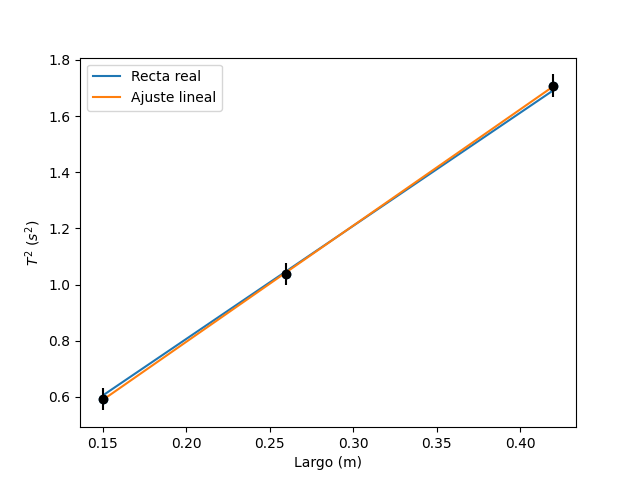
\includegraphics[width=0.6\linewidth]{gravedad.png}
    \caption{}   
    \label{fig:gravedad}
\end{figure}

Despejando g de la pendiente de la recta obtenemos: $g = 9.5 \pm 0.6 m/s^2$. Este parametro incluye a la gravedad real y a los errores de medicion del experimento.

Este informe abordará el desarrollo experimental, los métodos de análisis de los datos y la discusión de los resultados, con el fin de proporcionar una comprensión detallada del comportamiento oscilatorio de un péndulo y su relación con los parámetros físicos involucrados.

\section{Practica experimental}

\begin{figure}[H]
    \centering
    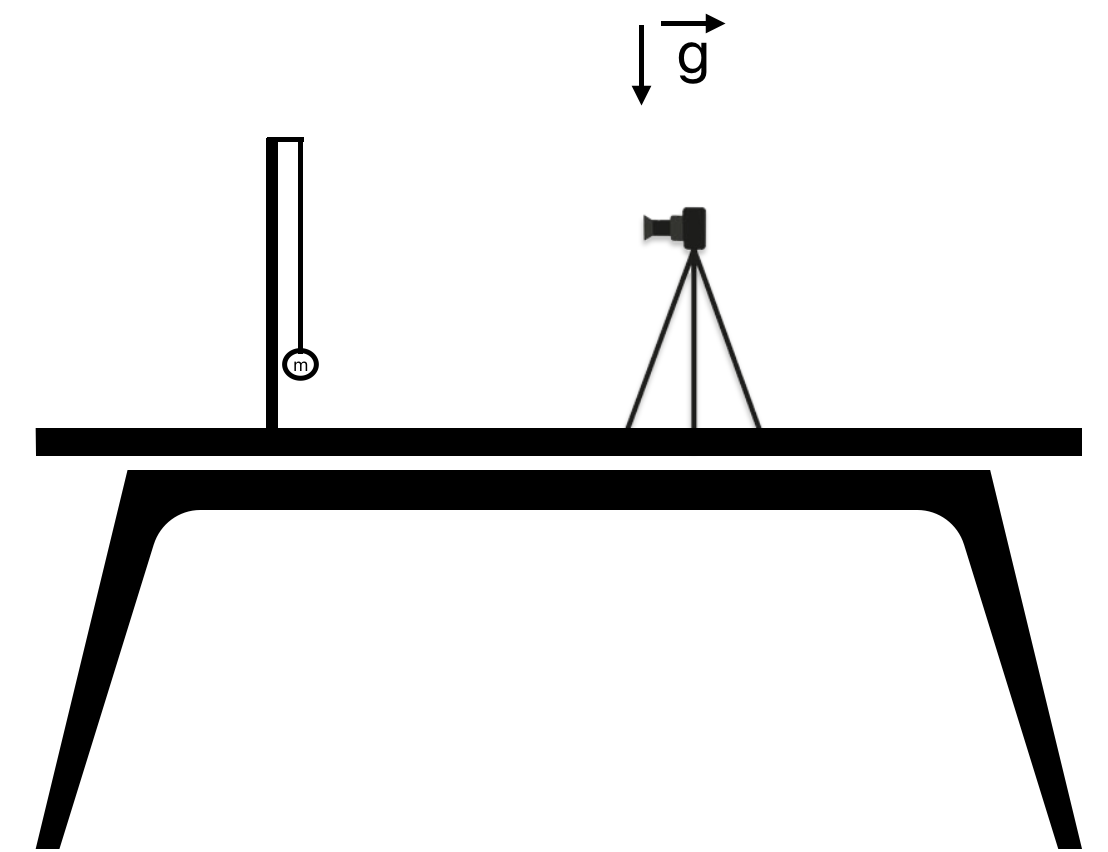
\includegraphics[width=0.6\linewidth]{esquema.png}
    \caption{Esquema del experimento donde m y el largo de la cuerda son variables}   
    \label{fig:esquema}
\end{figure}

Para llevar a cabo el experimento, dispusimos de un sistema compuesto por una masa, una soga y una cámara, que nos permitió construir un péndulo simple y grabar sus movimientos. El esquema del sistema se muestra en la Figura \ref{fig:esquema}. La masa y la longitud de la soga se pueden variar, lo que nos permitió experimentar con diferentes condiciones iniciales y observar sus efectos en el comportamiento del péndulo simple.

Para la adquisición de datos, utilizamos un teléfono para filmar los movimientos del péndulo y posteriormente analizamos los videos con el programa \textit{Tracker}, que permite seguir una masa específica en función del tiempo y registrar su posición en un sistema de coordenadas definido. Para obtener una referencia de distancia, colocamos una cinta métrica en el fondo de cada video, permitiendo al programa calibrar la relación entre píxeles y distancia real y, así, establecer la posición de la masa con precisión.

Una vez construido el sistema, procedimos con el experimento. Primero, mantuvimos una masa constante de $23 \pm 0.1 \, \text{g}$ y una longitud de soga de $42 \pm 0.1 \, \text{cm}$ y variamos los ángulos iniciales, utilizando valores de $\theta = \{55^\circ, 45^\circ, 25^\circ, 15^\circ, 10^\circ\} \pm 1^\circ$. Estos datos nos permitieron analizar el rango angular en el que se cumplen las condiciones de pequeñas oscilaciones, de modo que el péndulo se pueda modelar como un movimiento armónico simple.

Para el siguiente análisis, empleamos un largo fijo de $42 \pm 0.1 \, \text{cm}$, un ángulo inicial de $25^\circ \pm 1^\circ$ y variamos la masa, usando valores de $m = 5 \pm 1 \, \text{g}$, $m = 23 \pm 1 \, \text{g}$ y $m = 72 \pm 1 \, \text{g}$. El objetivo de este experimento fue estudiar el impacto de la masa en la frecuencia de oscilación del péndulo simple. Además, experimentamos manteniendo constantes la masa y el ángulo (con valores de $m = 23 \pm 0.1 \, \text{g}$ y $\theta = 25^\circ \pm 1^\circ$) y variando la longitud de la soga con valores de $L = 42 \pm 0.1 \, \text{cm}$, $L = 26 \pm 0.1 \, \text{cm}$ y $L = 15 \pm 0.1 \, \text{cm}$. Esto nos permitió analizar la dependencia de la frecuencia de oscilación con respecto a la longitud de la soga.

Finalmente, con los datos obtenidos y utilizando las ecuaciones de período y frecuencia del péndulo simple, calculamos la gravedad efectiva.


Los errores que tuvimos en cuenta fueron los siguientes:

\begin{itemize}
    \item Error en la medicion del largo de la soga: $\pm 0.1 cm$
    \item Error en la medicion del angulo inicial: $\pm 1^\circ$
    \item Error en la posicion de la bolita: $\pm 1 cm$ (radio de la bolita)
\end{itemize}

\section{Seguimiento de la trayectoria}



\section{Resultados}

Para los distintos angulos iniciales se obtuvieron los siguientes resultados:

\begin{figure}[H]
    \centering
    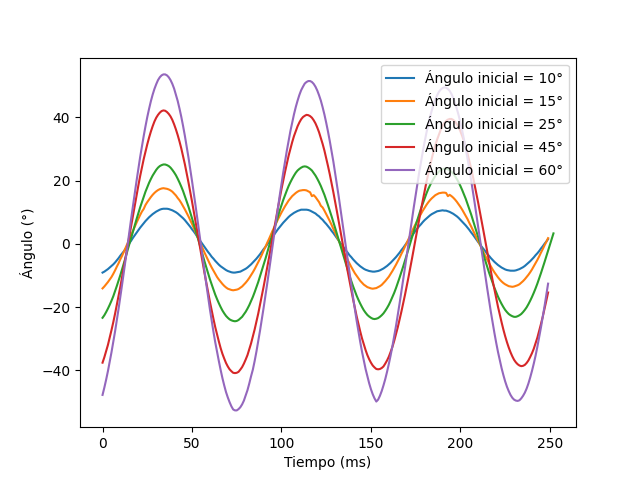
\includegraphics[width=0.6\linewidth]{angulos.png}
    \caption{Posicion de la masa en funcion del tiempo para distintos angulos iniciales}
    \label{fig:angulos}
\end{figure}

Se puede observar como la amplitud del movimiento no afecta la frecuencia del mismo. 

\begin{figure}[H]
    \centering
    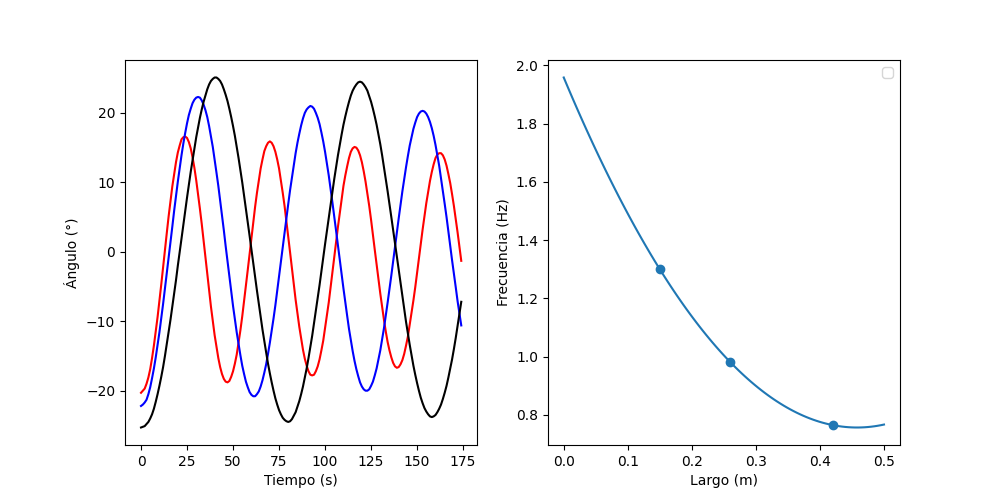
\includegraphics[width=0.6\linewidth]{largo.png}
    \caption{Posicion de la masa en funcion del tiempo para distintos largos de soga}
    \label{fig:largo}
\end{figure}

Se puede observar como el largo de la soga afecta la frecuencia del movimiento. A mayor largo, menor frecuencia. Esto se debe a que la bolita recorre una mayor distancia. Sabemos que la longitud de arco esta defenida como $d = r \theta$, por lo que a mayor longitud de soga, mayor longitud de arco recorre la bolita.

\begin{figure}[H]
    \centering
    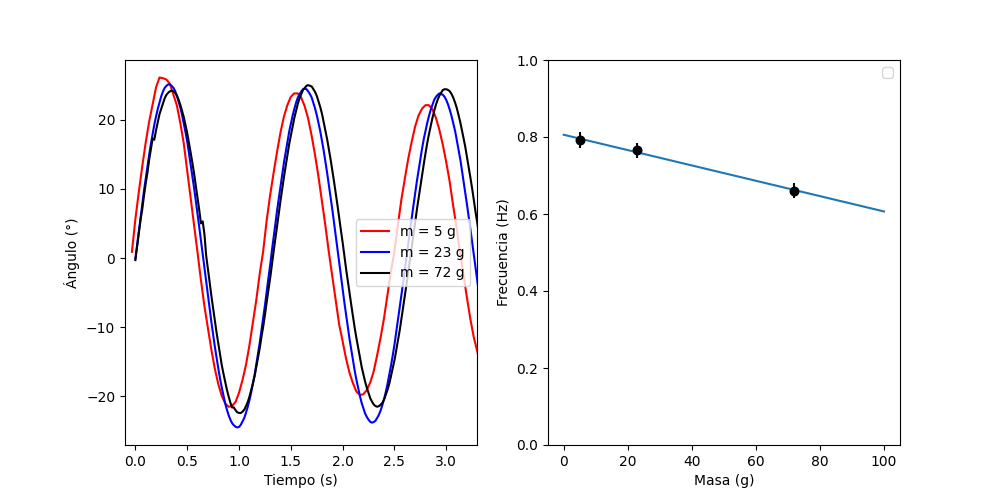
\includegraphics[width=0.6\linewidth]{peso.png}
    \caption{Posicion de la masa en funcion del tiempo para distintas masas}
    \label{fig:masa}
\end{figure}

Se puede observar como la masa de la bolita no afecta la frecuencia del movimiento excepto cuando la masa es chica. Esto se debe a en el experimento la soga no es perfectamente rigida, por lo que, al tener poca masa, el movimiento de la soga se deforma.

\end{document}